%!TEX root = ../crimson_throne_book_main.tex
% 2015-07-25
The companions' next destination is Yuuna's flat. Balian easily picks the lock and finds a small, but colorful room. There is no trace of Yuuna, there are no signs of a struggle, only the back window has been forced open. Nothing else is of any help to the young men, so they return to Eel's End to talk to Yuuna best friend, Danarella. The redhead has no idea where her Vudran colleague disappeared to, although she hopes her friend is okay. She might have fled to the mainland, but Danarella suspects that Yuuna would never do that without informing her. Maybe Yuuna's {\itshape stalker} knows more, she muses. She explains that Yuuna had a 'fan', a man who was probably in love with her and who regularly escorted her home after work. They jokingly called him her 'stalker', although he was quite a respectable man, a trainer at the Endrin military academy, called Janros Rainwater. Endrin military academy is a whitewashed building that acts as barracks and training grounds for a small garrison of both Korvosan guards and Sable Company trainees. This place does not just only drill soldiers and teach them new tricks and tactical insight, it also serves as a breeding ground for good relations between the Guard and the Sable Company. The trainees act as liaisons between the two military forces, allowing for joint operations and continued mutual support. The academy's location within the old wall of Fort Korvosa, at the foot of Garrison Hill, provides a more serene scenery than the chaotic streets of Old Docks and the cramped alleys of Bridgefront. Although there are signs of plundering and destruction here as well, they are less frequent and there are no decaying bodies on the ground or thugs about.\\

Double doors bar the entrance to the academy. A note has been nailed in the wood: {\itshape Academy closed - No entry} . Balian knocks loudly. The only reaction is a dog that starts barking inside, but no one answers the call. Since this building is so close to Vencarlo's house, the companions want to pay the fencing master a visit first. Maybe he knows his colleagues in this training center, so he might facilitate their access. Two blocks away stands Vencarlo's famed sword school, or at least, that is where it used to stand. The once-proud Orisini Academy is no more: the training facility has recently burnt to the ground. Fortunately, Vencarlo's living quarters still stand, nestled in the other corner of the compound. Puk's quick eyes pick up a line of smoke coming from the chimney, so the fencing expert is at home! When Balian knocks on the door, it clicks open from the impact of his blows. Why would Vencarlo leave his door unlocked? The companions draw their weapons and carefully enter the building. The ground floor is empty. If Vencarlo is still here, he is probably resting upstairs ... and if he isn't, the bedroom might just be the best place to find a trace. The stairs lead to a personal training room with a burning fireplace and two practice dummies in the far corners, to either side of the hearth. The exposed rafters give the room an open feel. There is one more door in here which can only lead to the bedroom. Puk's sixth sense warns him of a danger as\hyperref[fig:Red-Mantis-attack-in-Vencarlo-s-house-548844795]{ two shadows drop down from the beams above } . Their weird armor resembles the carapace of a scarlet insect and their blood-colored ant-like helmet completes the picture: Red Mantis assassins! \\

\begin{figure}[h]
	\centering
	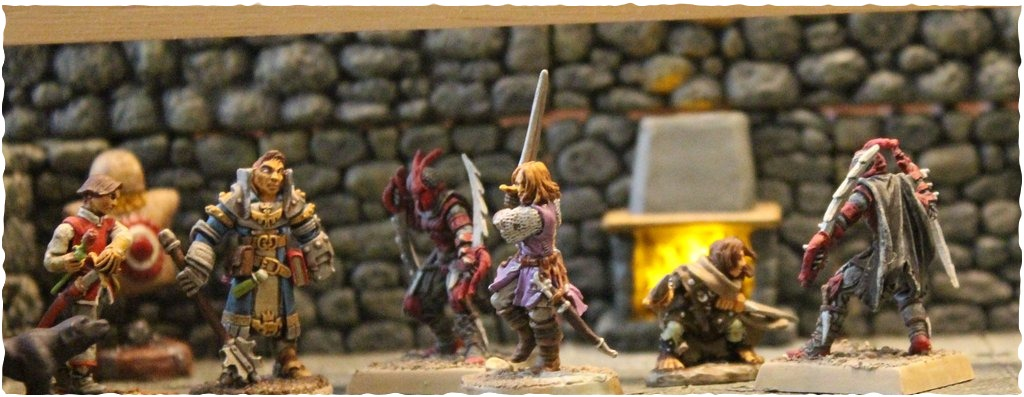
\includegraphics[width=0.4\textwidth]{images/Red-Mantis-attack-in-Vencarlo-s-house-548844795_mod.jpg}
	\caption{Red Mantis attack in Vencarlo's house}
	\label{fig:Red-Mantis-attack-in-Vencarlo-s-house-548844795}
\end{figure}

